\section{Approximate Riemann Solver}
Computing the exact solution to the riemann problem at the boundary of each of the cells is computationally expensive because it involves iterations over all of the cells for every timestep. In order to avoid doing this to be more computationally efficient, modern high resolution shock capturing schemes employ approximate riemann solvers to numerically approximate the solutions to the riemann problem at each of the boundaries. In my project, I used one of the simplest numerical flux functions, the FHLL flux. This flux approximates the solution to the local riemann problem as a two-state solution with an intermediate state in the middle. 
Approximate riemann solvers can be divided into complete and incomplete riemann solvers. Incomplete riemann solvers contain only a subset of the characteristic fields of exact solutions, whereas complete riemann solvers contain all of the characteristic fields of the exact solution. Complete riemann solvers are fully upwind and are able to capture any discontinuity or wave that forms during the evolution. Incomplete riemann solvers are usually only upwind with respect to the fastest possible waves that are produced in the riemann fan, but they are susceptible to losing information about intermediate waves. 
\subsection{The HLLE Numerical Solver}
This solver assmumes that after the decay of the initial discontinuity, only two waves propagate in two opposite directions with velocities $\lambda_L$ and $\lambda_R$, and a single constant state between them:
$$\bm{U}(x,t)=\begin{cases}
		\bm{U}_L , \quad x/t < \lambda_L \\
		\bm{U}^{HLLE} , \quad \lambda_L < x/t < \lambda_R \\
		\bm{U}_R , \quad x/t > \lambda_R
\end{cases}$$

\begin{figure}[h]
		\centering
		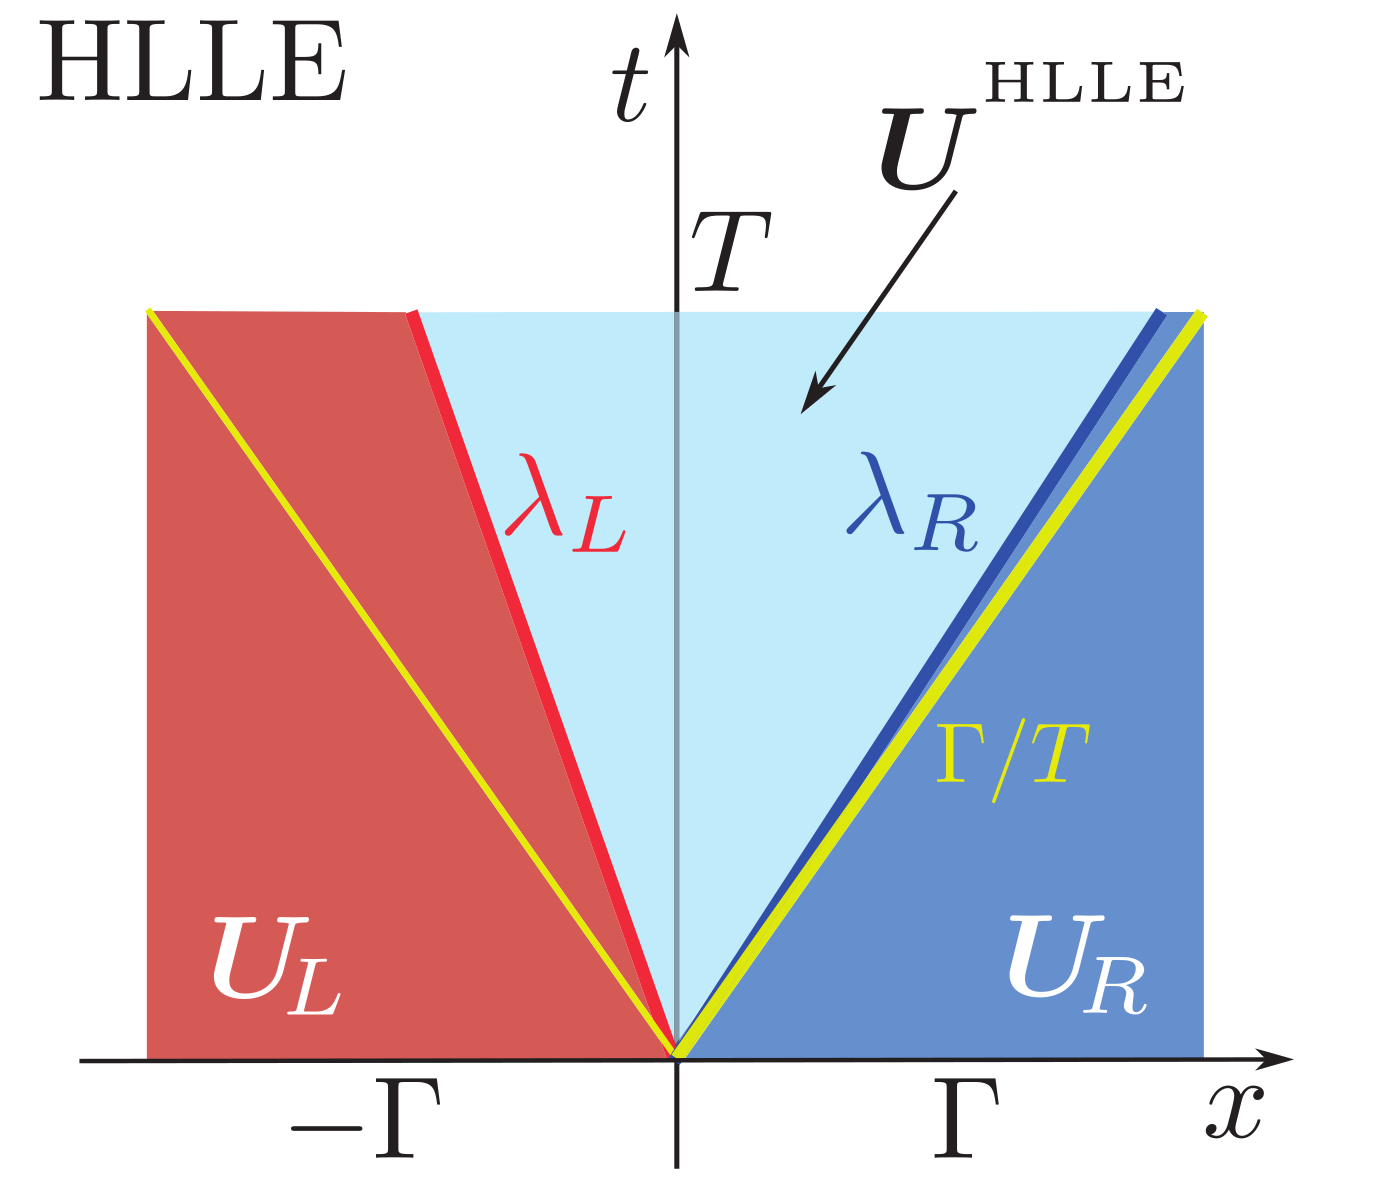
\includegraphics[scale=0.1]{HLLEFlux}
        \caption{Spacetime control Volume for the computation of the approximate HLLE FLux, \cite{rezzolla}}
\end{figure}

By applying the Rankine-Hugoniot conditions across the left and right waves, we can compute the constant state $\bm{U}^{HLLE}$, given that we know the signal speeds $\lambda_L$ and $\lambda_R$. Doing this, we obtain the HLLE flux:
$$F_{*}=\frac{\lambda_R\bm{F}_L-\lambda_L\bm{F}_R+\lambda_L\lambda_R(\bm{U}_R-\bm{U}_L)}{\lambda_R-\lambda_L}$$
We use the HLLE flux in the godnuov method using the logic:
$$\bm{F}^{HLLE}=\begin{cases}
		\bm{F}_L,\quad x/t < \lambda_L \\
		\bm{F}_{*},\quad \lambda_L < x/t < \lambda_R \\
		\bm{F}_R,\quad x/t > \lambda_R
\end{cases}$$
THis riemann solver has the pro of being very simple, and that it performs well at sonic rarefactions, but due to the fact that the middle waves are ignored in the solution, it shows exceissve smearing at contact  discontinuities. To use this riemann solver, we need to compute the wave speeds $\lambda_L$ and $\lambda_R$ in a way that is appropriate for special relativistic hydrodynamics:
$$\lambda_L = \min(0,\lambda_{-}(\bm{U}_L),\lambda_{-}(\bm{U}_R))$$
$$\lambda_R = \max(0, \lambda_{+}(\bm{U}_L),\lambda_{+}(\bm{U}_R))$$
where $\lambda_{-}$ and $\lambda_{+}$ are given by the appropriate eigenvalues of the jacobian matrix.

\subsection{The HLLC Numerical Solver }
Although the HLLE riemann solver is more simple, it suffers from strong limitations in terms of capturing contact and tangential waves. The HLLC riemann solver was introduced in order to restore the missing information about the intermediate contact discontinuity by using two intermediate states, $\bm{U}_{L_*}$ and $\bm{U}_{R_*}$. Using this, the complete solution is given by:
$$\bm{U}(x,t)=\begin{cases}
		\bm{U}_L, \quad x/t < \lambda_L\\
		\bm{U}_{L_*}, \quad \lambda_L < x/t < \lambda_C\\
		\bm{U}_{R_*},\quad \lambda_C < x/t < \lambda_R\\
		\bm{U}_R,\quad x/t > \lambda_R
\end{cases}$$
where $\lambda_L \leq 0 $ and $\lambda_R \geq 0$ are the smallest and largest of the characteristics of the solution to the local Riemann problem, and $\lambda_C$ is the speed of the contact discontinuity. The HLLC flux is given by:
$$\bm{F}^{HLLC}=\begin{cases}
		\bm{F}_L,\quad x/t < \lambda_L\\
		\bm{F}_{L_*},\quad \lambda_L < x/t < \lambda_C\\
		\bm{F}_{R_*},\quad \lambda_C < x/t < \lambda_R \\
		\bm{F}_R,\quad x/t > \lambda_R
\end{cases}$$
For this solution, it is required an estimate for the speeds $\lambda_L$, $\lambda_C$, and $\lambda_R$. For $\lambda_L$ and $\lambda_R$, one can use the same strategy used for the HLLE riemann solver, in which we used the largest and smallest eigenvalues of the jacobian matrix. An estimate for $\lambda_C$ is obtained as the speed of the contact discontinuity in the analytic solution of the two-rarefaction riemann solver. 
\begin{figure}[h]
		\centering
		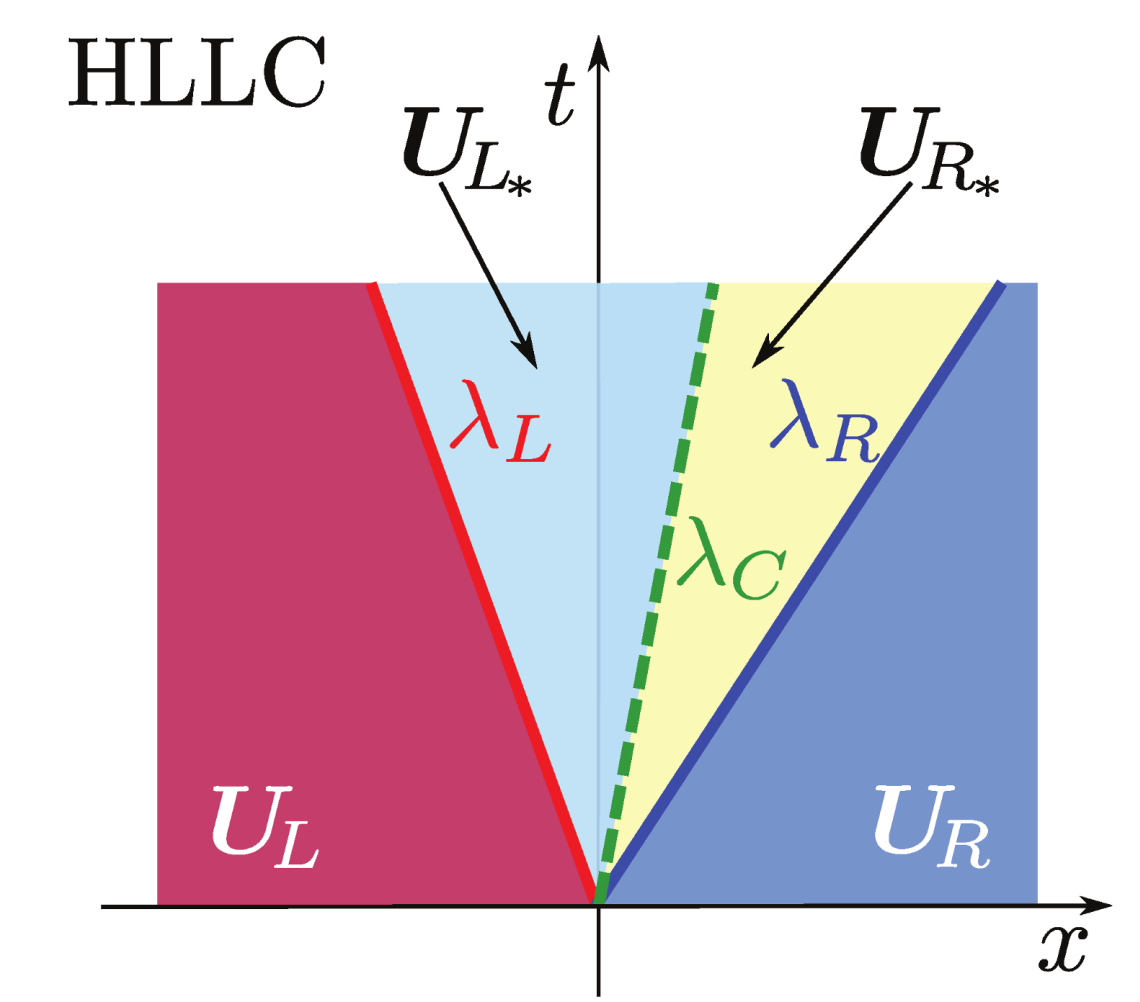
\includegraphics[scale=0.15]{HLLCFluxSolver}
        \caption{Spacetime control volume for the computation of approximate HLLC flux. This riemann fan is coposed of two waves with speeds $\lambda_L$ and $\lambda_R$ and an approximation to the contact discontinuity wave speed $\lambda_C$, \cite{rezzolla}}
\end{figure}

\subsection{My Code}
In my code, I implemented the HLLE riemann solver for the nonrelativistic and relativistic versions. In the future I would like to implement the HLLC riemann solver as well as other approximate riemann solvers and compare their performance. 
